\documentclass[a4paper]{article}

\usepackage{INTERSPEECH2021}
\usepackage{hyperref}
\usepackage{booktabs}
\usepackage{multicol}
\usepackage{graphicx}
\usepackage{amsmath}


% Put the lab number of the corresponding exercise
\title{NLU Course Project - Natural Language Understanding}
\name{Christian Dalvit (249988)}

\address{University of Trento}
\email{christian.dalvit@studenti.unitn.it}

\begin{document}

\maketitle

%Dear students, \\
%here you can find a complete description of the sections that you need to write for the mini-report. You have to write a mini-report of \textbf{max 1 page (references, tables and images are excluded from the count)} for each last exercise of labs 4 (LM), 5  (NLU) and 6 (SA). \textbf{Reports longer than 1 page will not be checked.} The purpose of this is to give you a way to report cleanly the results and give you space to describe what you have done and/or the originality that you have added to the exercise.\\
%\textbf{If you did the first part only, you have to just report the results in a table with a small description.}

\section{Introduction}
This project investigates the joint learning of intent classification and slot filling for natural language understanding using Long Short-Term Memory (LSTM) units and pre-trained BERT models as backbones. The LSTM-based models are enhanced with bidirectional architecture and dropout layers, while the BERT model is fine-tuned to improve performance. The effectiveness of these techniques is evaluated on the ATIS dataset using the $F_1$ score as a metric. The code of this project is made available on \href{https://github.com/chrisdalvit/nlu-assignment}{Github}.

\section{Implementation details}
All models in this project are implemented in PyTorch \cite{paszke2019pytorchimperativestylehighperformance}. The LSTM \cite{schmidhuber1997long} implementation from the \texttt{ModelIAS} class provided in Lab 5 is used as baseline. The baseline consists of an embedding layer, an LSTM unit, and a linear output layer, with the Adam optimizer employed for training. For the BERT \cite{devlin2019bertpretrainingdeepbidirectional} implementation, code snippets provided in Lab 5 are used as a reference.

\paragraph*{First Part}
In the first part, the baseline model is extended by adding bidirectionality to the LSTM unit. PyTorch provides a flag in its LSTM implementation to enable bidirectionality. When using a bidirectional LSTM, the input size of the linear output layer for slot filling must be doubled. Additionally, dropout layers are added before the embedding layer and the linear layer for intent classification. As PyTorch includes built-in implementations for dropout layers, their integration is straightforward.

\paragraph*{Second Part}
In the second part, pre-trained BERT models \cite{devlin2019bertpretrainingdeepbidirectional} are fine-tuned for slot filling and intent classification. The pre-trained models are accessed through the Huggingface library. Since Huggingface provides a convenient Python API, loading the different models was straightforward to implement. The project implementation supports loading weights for $\text{BERT}_{\text{LARGE}}$, $\text{BERT}_{\text{BASE}}$, $\text{BERT}_{\text{MEDIUM}}$, $\text{BERT}_{\text{SMALL}}$, $\text{BERT}_{\text{MINI}}$, and $\text{BERT}_{\text{TINY}}$ \cite{devlin2019bertpretrainingdeepbidirectional, turc2019wellreadstudentslearnbetter}. All models process uncased input text. An additional dropout layer is implemented and can optionally be applied before the final linear layer. A primary challenge when using models from the BERT family is tokenization. BERT models employ WordPiece \cite{wu2016googlesneuralmachinetranslation} tokenization, which can split a single input word into multiple subtokens. This creates a challenge for the slot filling task, as subtokens generates a corresponding hidden state. However, since slot filling requires only one label per word, it becomes necessary to either reduce the number of hidden states or adjust the labeling scheme to fit the subtokens. To address this, the approach proposed by Chen et al. \cite{chen2019bertjointintentclassification} is adopted in this project: only the first subtoken is used for slot filling. This is implemented by filtering the tokenized input text to select the first subtoken of each word.

\section{Results}
All models were evaluated on the ATIS dataset, with the $F_1$ score used to measure slot filling performance and accuracy used for intent classification. The evaluations were conducted on the Marzola cluster at the University of Trento.

\paragraph*{First Part}
In the first part, the baseline LSTM implementation was benchmarked against the bidirectional LSTM and the bidirectional LSTM with dropout. For all benchmarks in the first part, a hidden size of 200, an embedding size of 300, and a training batch size of 64 were used. Additionally, all LSTMs consisted of two layers, and training was performed over 200 epochs. No early stopping was applied for the first 5 epochs. After that, an early stopping patience of 3 epochs was used. Each setup was run 10 times. Table \ref{tab:slot_filling_part1} reports the mean $F_1$ score for slot filling over the runs. Bidirectionality improved the baseline performance by approximately 3 points. Adding dropout achieved the best overall performance. The best-performing Adam configuration was also tested with SGD, which resulted in a slight performance drop. Table \ref{tab:intent_accuracy_part1} shows the mean accuracy for intent classification over the runs. Incorporating bidirectionality and dropout into the baseline both improved accuracy. Similar to the slot filling task, experiments with the SGD optimizer resulted in a slight decline in performance compared to Adam. Figure \ref{fig:part_1_convergence} illustrates the convergence of the $F_1$ score over the training epochs. The addition of bidirectionality and dropout led to faster and more stable convergence of the $F_1$ metric. 
The experiments show that bidirectionality significantly improves performance in slot filling and intent classification tasks. 

\paragraph*{Second Part}
For the second part, the $\text{BERT}_{\text{BASE}}$ implementation was used as the baseline. All models were trained with a batch size of 64 for 10 epochs. For $\text{BERT}_{\text{BASE}}$ and $\text{BERT}_{\text{LARGE}}$, experiments with a 0.2 dropout rate were conducted.Table \ref{tab:slot_filling_part2} shows the $F_1$ score for slot filling across the different models. The results indicate that smaller learning rates, such as $5 \times 10^{-5}$, are better suited for larger models like $\text{BERT}_{\text{LARGE}}$ and $\text{BERT}_{\text{BASE}}$, which fail to produce meaningful results at higher learning rates, such as $1 \times 10^{-4}$. Conversely, smaller BERT models perform better with higher learning rates, such as $1 \times 10^{-4}$. Although $\text{BERT}_{\text{LARGE}}$ with dropout achieves the best performance, it is worth mentioning that some smaller models, such as $\text{BERT}_{\text{MEDIUM}}$ and $\text{BERT}_{\text{MINI}}$, perform only slightly worse. Table \ref{tab:intent_accuracy_part2} presents the accuracy for intent classification across the different models. Most conclusions drawn from Table \ref{tab:slot_filling_part2} also apply to this task. The best learning rates are $1 \times 10^{-4}$ and $5 \times 10^{-5}$, with larger models tending to perform better at smaller learning rates and smaller models working better at higher learning rates. $\text{BERT}_{\text{LARGE}}$ shows a significant performance drop at a learning rate of $1 \times 10^{-4}$. For intent classification, it is also worth noting that smaller models like $\text{BERT}_{\text{MEDIUM}}$ and $\text{BERT}_{\text{MINI}}$ perform only slightly worse than the best-performing model, $\text{BERT}_{\text{LARGE}}$ with dropout.

\begin{table}
  \caption{Mean Slot Filling $F_1$ scores in the first part}
  \label{tab:slot_filling_part1}
  \begin{tabular}{l|c c c c}
    \toprule
    \textbf{Model} & \multicolumn{4}{c}{\textbf{Learning rate} } \\
    \midrule
    \textit{Adam optimizer} & \textbf{1e-4} & \textbf{5e-4} & \textbf{1e-3} & \textbf{5e-3} \\
    \midrule
    LSTM & ${90.25}^*$ & \underline{91.24} & 91.04 & 91.13 \\
    LSTM + BiD & 91.79 & 93.54 & 93.87 & \underline{94.43}\\
    LSTM + BiD + DR0.2 & 92.58 & 93.90 & 94.39 & \textbf{94.60} \\
    \toprule
    \textit{SGD optimizer} & \textbf{4}	& \textbf{5} & \textbf{6} & \textbf{7} \\
    \midrule
    LSTM + BiD + DR0.2 & \textbf{94.07} & 93.75 & 93.88 & 93.79 \\  
    \bottomrule
  \end{tabular}
  \begin{minipage}{7.5cm}
    \vspace{0.1cm}
    * This value was computed on only 7 runs, because 3 runs produced an error and therefore having an $F_1$ score of 0.\\
    Note: Underlined values show the best $F_1$ score of a model and the bold value shows the best $F_1$ score over all models for a given optimizer.
  \end{minipage}
\end{table}

\begin{table}[htbp]
  \caption{Mean Intent Classification accuracy in the first part}
  \label{tab:intent_accuracy_part1}
  \begin{tabular}{l|c c c c}
    \toprule
    \textbf{Model} & \multicolumn{4}{c}{\textbf{Learning rate} } \\
    \midrule
    \textit{Adam optimizer} & \textbf{1e-4} & \textbf{5e-4} & \textbf{1e-3} & \textbf{5e-3} \\
    \midrule
    LSTM & ${92.68}^*$ & \underline{92.69} & 92.19 & 91.03 \\
    LSTM + BiD & 94.82 & 95.70 & \underline{96.10} & 95.50 \\
    LSTM + BiD + DR0.2 & 95.42 & \textbf{96.15} & 96.08 & 95.69 \\
    \toprule
    \textit{SGD optimizer} & \textbf{4}	& \textbf{5} & \textbf{6} & \textbf{7} \\
    \midrule
    LSTM + BiD + DR0.2 & 95.40	& 95.60 & 95.50 & \textbf{95.68}\\
    \bottomrule
  \end{tabular}
  \begin{minipage}{7.5cm}
    \vspace{0.1cm}
    * This value was computed on only 7 runs, because 3 runs produced an error and therefore having an intent accuracy of 0.\\
    Note: Underlined values show the best classification accuracy of a model and the bold value shows the best classification accuracy over all models for a given optimizer. 
  \end{minipage}
\end{table}

\begin{figure}[htbp]
  \centering
  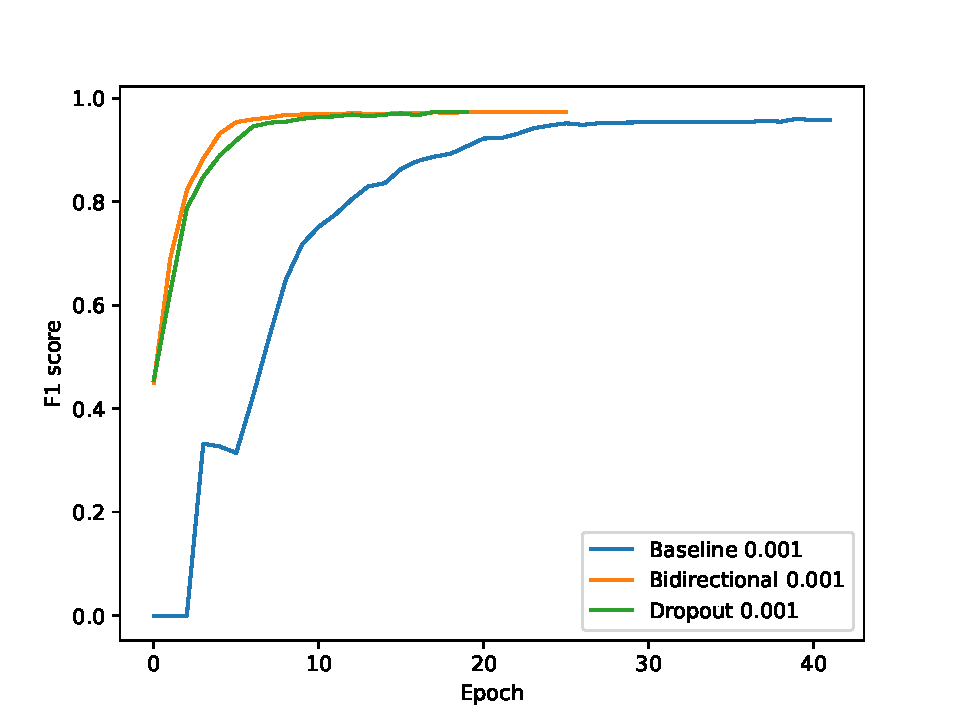
\includegraphics[width=0.5\textwidth]{part1_convergence.pdf}
  \caption{The $F_1$ score convergence over the training epochs of selected models in the first part. The labels denote the model name with the learning rate}
  \label{fig:part_1_convergence}  
\end{figure}

\begin{table}[ht!]
  \caption{Slot Filling $F_1$ scores in the second part}
  \label{tab:slot_filling_part2}
  \centering
  \begin{tabular}{l|c c c}
    \toprule
    \textbf{Model} & \multicolumn{3}{c}{\textbf{Learning rate} } \\
    \midrule
    \textit{Adam optimizer} & \textbf{1e-5} & \textbf{5e-5} & \textbf{1e-4} \\
    \midrule
    $\text{BERT}_{\text{LARGE}}$ & 92.73 & \underline{95.55} & $0.00^*$ \\
    $\text{BERT}_{\text{LARGE}}$ + DR0.2 & 92.01 & \textbf{95.66} & $0.00^*$ \\
    $\text{BERT}_{\text{BASE}}$ & 90.74 & \underline{95.23} & 94.71 \\
    $\text{BERT}_{\text{BASE}}$ + DR0.2 & 89.67 & 94.43 & \underline{95.27} \\
    $\text{BERT}_{\text{MEDIUM}}$ & 85.51 & 94.41 & \underline{94.78} \\
    $\text{BERT}_{\text{SMALL}}$ & 75.06 & 87.92 & \underline{91.83} \\
    $\text{BERT}_{\text{MINI}}$ & 80.92 & 93.33 & \underline{94.94} \\
    $\text{BERT}_{\text{TINY}}$ & 40.41 & 76.71 & \underline{82.01} \\
    \bottomrule
  \end{tabular}
  \begin{minipage}{7.5cm}
    \vspace{0.1cm}
    * The $\text{BERT}_{\text{LARGE}}$ does not produce meaningful slot filling results for this learning rate and therefore produces a $F_1$ score of 0.\\
    Note: Underlined values show the best $F_1$ score of a model and the bold value shows the best $F_1$ score over all models.
  \end{minipage}
\end{table}

\begin{table}[ht!]
  \caption{Intent Classification accuracy in the second part}
  \label{tab:intent_accuracy_part2}
  \centering
  \begin{tabular}{l|c c c}
    \toprule
    \textbf{Model} & \multicolumn{3}{c}{\textbf{Learning rate} } \\
    \midrule
    \textit{Adam optimizer} & \textbf{1e-5} & \textbf{5e-5} & \textbf{1e-4} \\
    \midrule
    $\text{BERT}_{\text{LARGE}}$ & 97.31 & \underline{97.42} & 70.77 \\
    $\text{BERT}_{\text{LARGE}}$ + DR0.2 & 97.42 & \textbf{97.76} & 70.77 \\
    $\text{BERT}_{\text{BASE}}$ & 94.96 & 97.31 & \textbf{97.76} \\
    $\text{BERT}_{\text{BASE}}$ + DR0.2 & 92.05 & \underline{97.65} & 97.09\\
    $\text{BERT}_{\text{MEDIUM}}$ & 93.17 & 96.53 & \underline{97.65} \\
    $\text{BERT}_{\text{SMALL}}$ & 93.06 & \underline{96.86} & 96.64 \\
    $\text{BERT}_{\text{MINI}}$ & 83.43 & 95.52 & \underline{97.42} \\
    $\text{BERT}_{\text{TINY}}$ & 70.88 & 88.80 & \underline{92.16} \\
    \bottomrule
  \end{tabular}
  \begin{minipage}{7.5cm}
    \vspace{0.1cm}
    Note: Underlined values show the best classification accuracy of a model and the bold value shows the best classification accuracy over all models. 
  \end{minipage}
\end{table}
\bibliographystyle{IEEEtran}
\bibliography{mybib}
\end{document}
